\section{The case $[5, 8]_3$}
\begin{theorem}
  Let $p = (p_3, p_4, p_5, \dots, p_n)$ be a given sequence satisfying equation \ref{eq_valence_3}, then there exists $r \in \nats$ for which $p + r [2 \times 5, 8]_3$ is $3$-realizable.
  \begin{proof}
    The proof is unsuprisingly similiar to the last one given. Again one chooses a realization by the classical Eberhards Theorem \ref{thm_eberhard}(\ref{thm_eberhard_3}) and substitutes the surplus of hexagons by two pentagons and one octagon. Seperating the faces in a kind of different way then before, this gives enough space for this substitution. The separation consists of an ring of pentagons around each polygon of the realization followed by a ring of octagons and fitting in the emerging holes another round of pentagons (equal to the number of pentagons and octagons in the previous rings as to have a discrete curvature of zero). This process is depicted below:

    \begin{figure}[htpp]
      \centering
      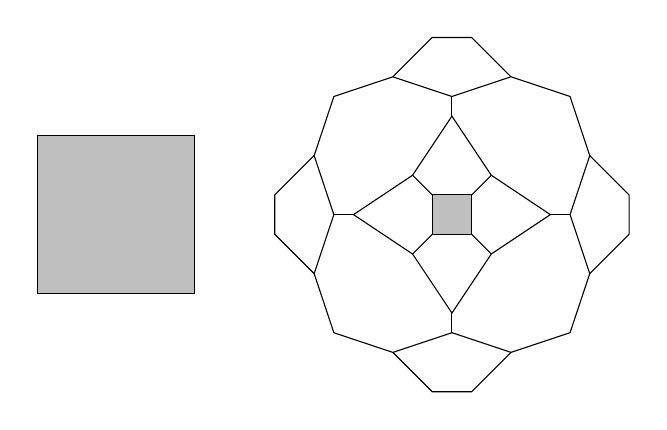
\begin{tikzpicture}
        \matrix (m) [ column sep=1cm] {

          \begin{scope} 
            \filldraw[fill=gray!50!white] (-1, -1) -- (1, -1) -- (1, 1) -- (-1, 1) -- (-1, -1);
          \end{scope}
          &
          \begin{scope}[scale=0.25] 
            \draw (-6, 0) -- (-7, -3) -- (-6, -6) -- (-3, -7) -- (0, -6) -- (3, -7) -- (6, -6) -- (7, -3) -- (6, 0) -- (7, 3) -- (6, 6) -- (3, 7) -- (0, 6) -- (-3, 7) -- (-6, 6) -- (-7, 3) -- (-6, 0);
            \draw (-5, 0) -- (-6, 0);
            \draw (0, -5) -- (0, -6);
            \draw (5, 0) -- (6, 0);
            \draw (0, 5) -- (0, 6);

            \draw (-5, 0) -- (-2, -2) -- (0, -5) -- (2, -2) -- (5, 0) -- (2, 2) -- (0, 5) -- (-2, 2) -- (-5, 0);
            \draw (-2, -2) -- (-1, -1);
            \draw (2, -2) -- (1, -1);
            \draw (2, 2) -- (1, 1);
            \draw (-2, 2) -- (-1, 1);
            
            \filldraw[fill=gray!50!white] (-1, -1) -- (1, -1) -- (1, 1) -- (-1, 1) -- (-1, -1);
            \draw (-7, -3) -- (-9, -1) -- (-9, 1) -- (-7, 3);
            \draw ( 7, -3) -- ( 9, -1) -- ( 9, 1) -- ( 7, 3);
            \draw (-3, -7) -- (-1, -9) -- (1, -9) -- (3, -7);
            \draw (3, 7) -- (1, 9) -- (-1, 9) -- (-3, 7);

          \end{scope}
          
          \\
        };
      \end{tikzpicture}
    \end{figure}


    \begin{figure}[htpp]
      \centering
      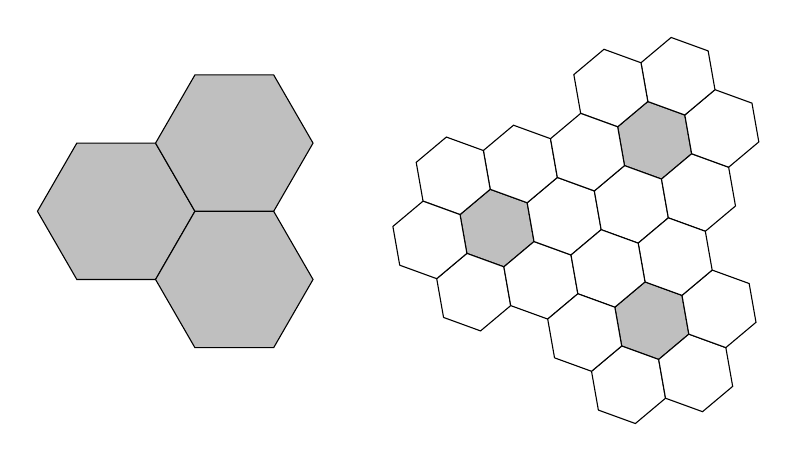
\begin{tikzpicture}
        \matrix (m) [ column sep=1cm] {
          \begin{scope}[xscale=1.0, yscale=0.866]
            \filldraw[fill=gray!50!white] (0, 1) -- ++(0.5, -1) -- ++(1, 0) -- ++(0.5, 1) -- ++(-0.5, 1) -- ++(-1, 0) -- ++(-0.5, -1);
            \filldraw[fill=gray!50!white] (1.5, 0) -- ++(0.5, -1) -- ++(1, 0) -- ++(0.5, 1) -- ++(-0.5, 1) -- ++(-1, 0) -- ++(-0.5, -1);
            \filldraw[fill=gray!50!white] (1.5, 2) -- ++(0.5, -1) -- ++(1, 0) -- ++(0.5, 1) -- ++(-0.5, 1) -- ++(-1, 0) -- ++(-0.5, -1);
          \end{scope}
          &


          \begin{scope}[rotate=40, xscale=1.0, yscale=0.866, scale=0.5] 
            \filldraw[fill=gray!50!white] (0, 1) -- ++(0.5, -1) -- ++(1, 0) -- ++(0.5, 1) -- ++(-0.5, 1) -- ++(-1, 0) -- ++(-0.5, -1);
            \filldraw[fill=white] (-1.5, 0) -- ++(0.5, -1) -- ++(1, 0) -- ++(0.5, 1) -- ++(-0.5, 1) -- ++(-1, 0) -- ++(-0.5, -1);
            \filldraw[fill=white] (0, -1) -- ++(0.5, -1) -- ++(1, 0) -- ++(0.5, 1) -- ++(-0.5, 1) -- ++(-1, 0) -- ++(-0.5, -1);
            \filldraw[fill=white] (1.5, 0) -- ++(0.5, -1) -- ++(1, 0) -- ++(0.5, 1) -- ++(-0.5, 1) -- ++(-1, 0) -- ++(-0.5, -1);
            \filldraw[fill=white] (1.5, 2) -- ++(0.5, -1) -- ++(1, 0) -- ++(0.5, 1) -- ++(-0.5, 1) -- ++(-1, 0) -- ++(-0.5, -1);
            \filldraw[fill=white] (0, 3) -- ++(0.5, -1) -- ++(1, 0) -- ++(0.5, 1) -- ++(-0.5, 1) -- ++(-1, 0) -- ++(-0.5, -1);
            \filldraw[fill=white] (-1.5, 2) -- ++(0.5, -1) -- ++(1, 0) -- ++(0.5, 1) -- ++(-0.5, 1) -- ++(-1, 0) -- ++(-0.5, -1);

            \filldraw[fill=gray!50!white] (4.5, 0) -- ++(0.5, -1) -- ++(1, 0) -- ++(0.5, 1) -- ++(-0.5, 1) -- ++(-1, 0) -- ++(-0.5, -1);
            \filldraw[fill=white] (3, -1) -- ++(0.5, -1) -- ++(1, 0) -- ++(0.5, 1) -- ++(-0.5, 1) -- ++(-1, 0) -- ++(-0.5, -1);
            \filldraw[fill=white] (4.5, -2) -- ++(0.5, -1) -- ++(1, 0) -- ++(0.5, 1) -- ++(-0.5, 1) -- ++(-1, 0) -- ++(-0.5, -1);
            \filldraw[fill=white] (6, -1) -- ++(0.5, -1) -- ++(1, 0) -- ++(0.5, 1) -- ++(-0.5, 1) -- ++(-1, 0) -- ++(-0.5, -1);
            \filldraw[fill=white] (6, 1) -- ++(0.5, -1) -- ++(1, 0) -- ++(0.5, 1) -- ++(-0.5, 1) -- ++(-1, 0) -- ++(-0.5, -1);
            \filldraw[fill=white] (4.5, 2) -- ++(0.5, -1) -- ++(1, 0) -- ++(0.5, 1) -- ++(-0.5, 1) -- ++(-1, 0) -- ++(-0.5, -1);
            \filldraw[fill=white] (3, 1) -- ++(0.5, -1) -- ++(1, 0) -- ++(0.5, 1) -- ++(-0.5, 1) -- ++(-1, 0) -- ++(-0.5, -1);
            
            \filldraw[fill=gray!50!white] (1.5, -4) -- ++(0.5, -1) -- ++(1, 0) -- ++(0.5, 1) -- ++(-0.5, 1) -- ++(-1, 0) -- ++(-0.5, -1);
            \filldraw[fill=white] (0, -5) -- ++(0.5, -1) -- ++(1, 0) -- ++(0.5, 1) -- ++(-0.5, 1) -- ++(-1, 0) -- ++(-0.5, -1);
            \filldraw[fill=white] (1.5, -6) -- ++(0.5, -1) -- ++(1, 0) -- ++(0.5, 1) -- ++(-0.5, 1) -- ++(-1, 0) -- ++(-0.5, -1);
            \filldraw[fill=white] (3, -5) -- ++(0.5, -1) -- ++(1, 0) -- ++(0.5, 1) -- ++(-0.5, 1) -- ++(-1, 0) -- ++(-0.5, -1);
            \filldraw[fill=white] (3, -3) -- ++(0.5, -1) -- ++(1, 0) -- ++(0.5, 1) -- ++(-0.5, 1) -- ++(-1, 0) -- ++(-0.5, -1);
            \filldraw[fill=white] (1.5, -2) -- ++(0.5, -1) -- ++(1, 0) -- ++(0.5, 1) -- ++(-0.5, 1) -- ++(-1, 0) -- ++(-0.5, -1);
            \filldraw[fill=white] (0, -3) -- ++(0.5, -1) -- ++(1, 0) -- ++(0.5, 1) -- ++(-0.5, 1) -- ++(-1, 0) -- ++(-0.5, -1);
          \end{scope};
          \\
        };
      \end{tikzpicture}
    \end{figure}


    One now chooses a set $S$ of hexagons one wants to keep, $|S| = p_6$. Each hexagon not in $S$ and the surrounding six hexagons are replaced by the following structure: 

    \begin{figure}[htpp]
      \centering
      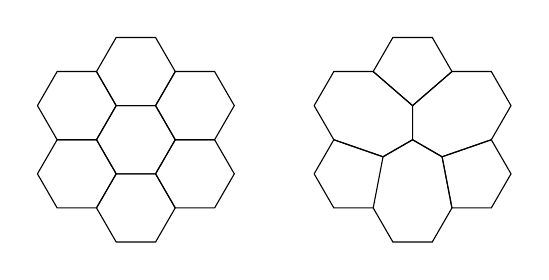
\begin{tikzpicture}
        \matrix (m) [ column sep=1cm] {
          \begin{scope}[xscale=1.0, yscale=0.866, scale=0.5]
            \draw (0, 1) -- ++(0.5, -1) -- ++(1, 0) -- ++(0.5, 1) -- ++(-0.5, 1) -- ++(-1, 0) -- ++(-0.5, -1);
            \draw (-1.5, 0) -- ++(0.5, -1) -- ++(1, 0) -- ++(0.5, 1) -- ++(-0.5, 1) -- ++(-1, 0) -- ++(-0.5, -1);
            \draw (0, -1) -- ++(0.5, -1) -- ++(1, 0) -- ++(0.5, 1) -- ++(-0.5, 1) -- ++(-1, 0) -- ++(-0.5, -1);
            \draw (1.5, 0) -- ++(0.5, -1) -- ++(1, 0) -- ++(0.5, 1) -- ++(-0.5, 1) -- ++(-1, 0) -- ++(-0.5, -1);
            \draw (1.5, 2) -- ++(0.5, -1) -- ++(1, 0) -- ++(0.5, 1) -- ++(-0.5, 1) -- ++(-1, 0) -- ++(-0.5, -1);
            \draw (0, 3) -- ++(0.5, -1) -- ++(1, 0) -- ++(0.5, 1) -- ++(-0.5, 1) -- ++(-1, 0) -- ++(-0.5, -1);
            \draw (-1.5, 2) -- ++(0.5, -1) -- ++(1, 0) -- ++(0.5, 1) -- ++(-0.5, 1) -- ++(-1, 0) -- ++(-0.5, -1);
          \end{scope};

          &

          \begin{scope}[xscale=1.0, yscale=0.866, scale=0.5] 
            \draw (-1.5, 0) -- ++(0.5, -1) -- ++(1, 0) -- ++(0.25, 1.5) -- ++(-1.25, 0.5) -- ++(-0.5, -1);
            \draw (0, -1) -- ++(0.5, -1) -- ++(1, 0) -- ++(0.5, 1) -- ++(-0.25, 1.5) -- ++(-0.75, 0.5) -- ++(-0.75, -0.5);
            \draw (1.75, 0.5) -- ++(0.25, -1.5) -- ++(1, 0) -- ++(0.5, 1) -- ++(-0.5, 1) -- ++(-1.25, -0.5);
            \draw (1, 1) -- ++(0.75, -0.5) -- ++(1.25, 0.5) -- ++(0.5, 1) -- ++(-0.5, 1) -- ++(-1, 0) -- ++(-1, -1);
            \draw (0, 3) -- ++(1, -1) -- ++(1, 1) -- ++(-0.5, 1) -- ++(-1, 0) -- ++(-0.5, -1);
            \draw (-1.5, 2) -- ++(0.5, -1) -- ++(1.25, -0.5) -- ++(0.75, 0.5) -- ++(0, 1) -- ++(-1, 1) -- ++(-1, 0) -- ++(-0.5, -1);
          \end{scope};
          
          \\
        };
      \end{tikzpicture}
    \end{figure}

    For the remaining hexagons and all other kinds of polygons this ring structure is replaced differently, for each $n$-gon $n$ pentagons and $n$ heptagons replace the ring of hexagons:

    \begin{figure}[htpp]
      \centering
      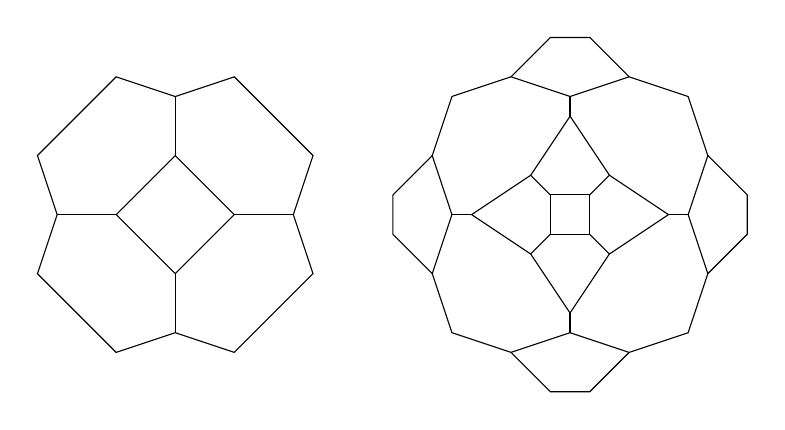
\begin{tikzpicture}
        \matrix (m) [ column sep=1cm] {

          \begin{scope}[scale=0.25] 
            \draw (-3, 0) -- (0, -3) -- (3, 0) -- (0, 3) -- (-3, 0);
            \draw (-3, 0) -- (-6, 0);
            \draw (0, -3) -- (0, -6);
            \draw (3, 0) -- (6, 0);
            \draw (0, 3) -- (0, 6);
            \draw (-6, 0) -- (-7, -3) -- (-3, -7) -- (0, -6) -- (3, -7) -- (7, -3) -- (6, 0) -- (7, 3) -- (3, 7) -- (0, 6) -- (-3, 7) -- (-7, 3) -- (-6, 0);
          \end{scope}
          &
          \begin{scope}[scale=0.25] 
            \draw (-6, 0) -- (-7, -3) -- (-6, -6) -- (-3, -7) -- (0, -6) -- (3, -7) -- (6, -6) -- (7, -3) -- (6, 0) -- (7, 3) -- (6, 6) -- (3, 7) -- (0, 6) -- (-3, 7) -- (-6, 6) -- (-7, 3) -- (-6, 0);
            \draw (-5, 0) -- (-6, 0);
            \draw (0, -5) -- (0, -6);
            \draw (5, 0) -- (6, 0);
            \draw (0, 5) -- (0, 6);

            \draw (-5, 0) -- (-2, -2) -- (0, -5) -- (2, -2) -- (5, 0) -- (2, 2) -- (0, 5) -- (-2, 2) -- (-5, 0);
            \draw (-2, -2) -- (-1, -1);
            \draw (2, -2) -- (1, -1);
            \draw (2, 2) -- (1, 1);
            \draw (-2, 2) -- (-1, 1);
            
            \draw (-1, -1) -- (1, -1) -- (1, 1) -- (-1, 1) -- (-1, -1);
            \draw (-7, -3) -- (-9, -1) -- (-9, 1) -- (-7, 3);
            \draw ( 7, -3) -- ( 9, -1) -- ( 9, 1) -- ( 7, 3);
            \draw (-3, -7) -- (-1, -9) -- (1, -9) -- (3, -7);
            \draw (3, 7) -- (1, 9) -- (-1, 9) -- (-3, 7);

          \end{scope}
          
          \\
        };
      \end{tikzpicture}
    \end{figure}
    This finishes the proof.
  \end{proof}
\end{theorem}


